\section{Exercise 5: Cumulocity}
Exercise number five is about \textit{Cumulocity}. There are three tasks defined in the sheet about how to 
use some features of \textit{Cumulocity} portal.

\subsection{Task 1: Dashboards}
The first task is about creating a dashboard in \textit{Cumulocity} portal. Therefore it was required to 
connect the smartphone to \textit{Cumulocity} and install the \textit{Cumulocity} app on the smartphone.
After this the smartphone could be used to collect data like the battery level, the current location gyroscope 
and accelerometer data. This data was then visualized in a dashboard in the \textit{Cumulocity} portal.

On the picture bellow you can see the dashboard as well as my location during the time i was working on this
exercise.
\begin{figure}[H]
    \centering
    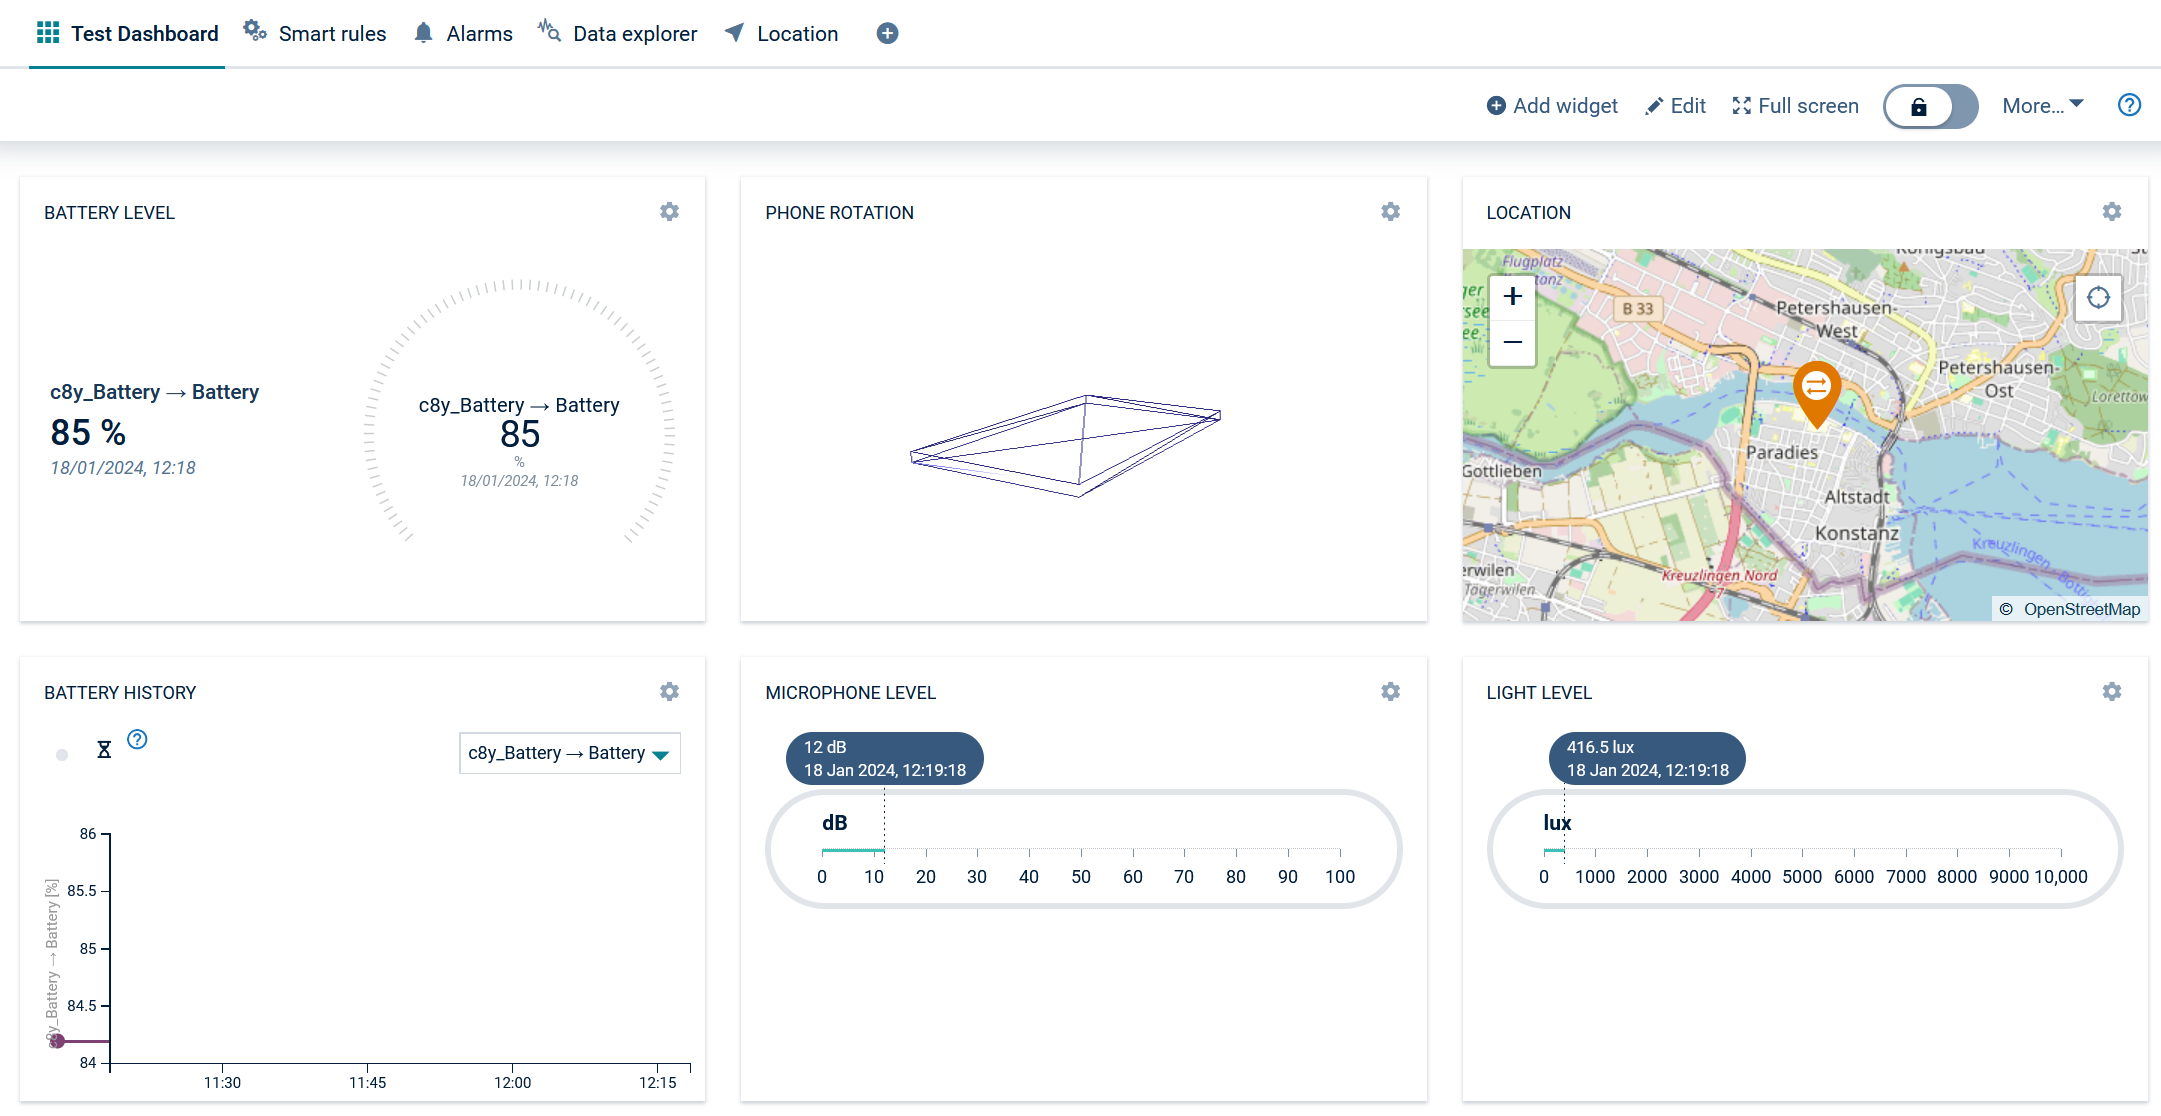
\includegraphics[width=1\textwidth]{exercise_cummolocity/task_1_dashboard.png}
    \caption{Cumulocity Dashboard}
    \label{fig:cumulocity_dashboard}
\end{figure}

\subsection{Task 2: Smart Rules}
The second task is about creating a smart rule in \textit{Cumulocity} portal. 
There we will use our already connected smartphone to trigger an alarm when it is upright or level.
Like in the first task this was straight forward following the instructions on the tutorial page.
As i did not read further at the task where the vibration alarm was set up to the next section, where it 
was described how to stop the vibration alarm again, my phone turned into a device we do not want to go 
to deep into detail here. Anyway bellow you will see the crated smart rule and the alarm which was triggered.

\begin{figure}[H]
    \centering
    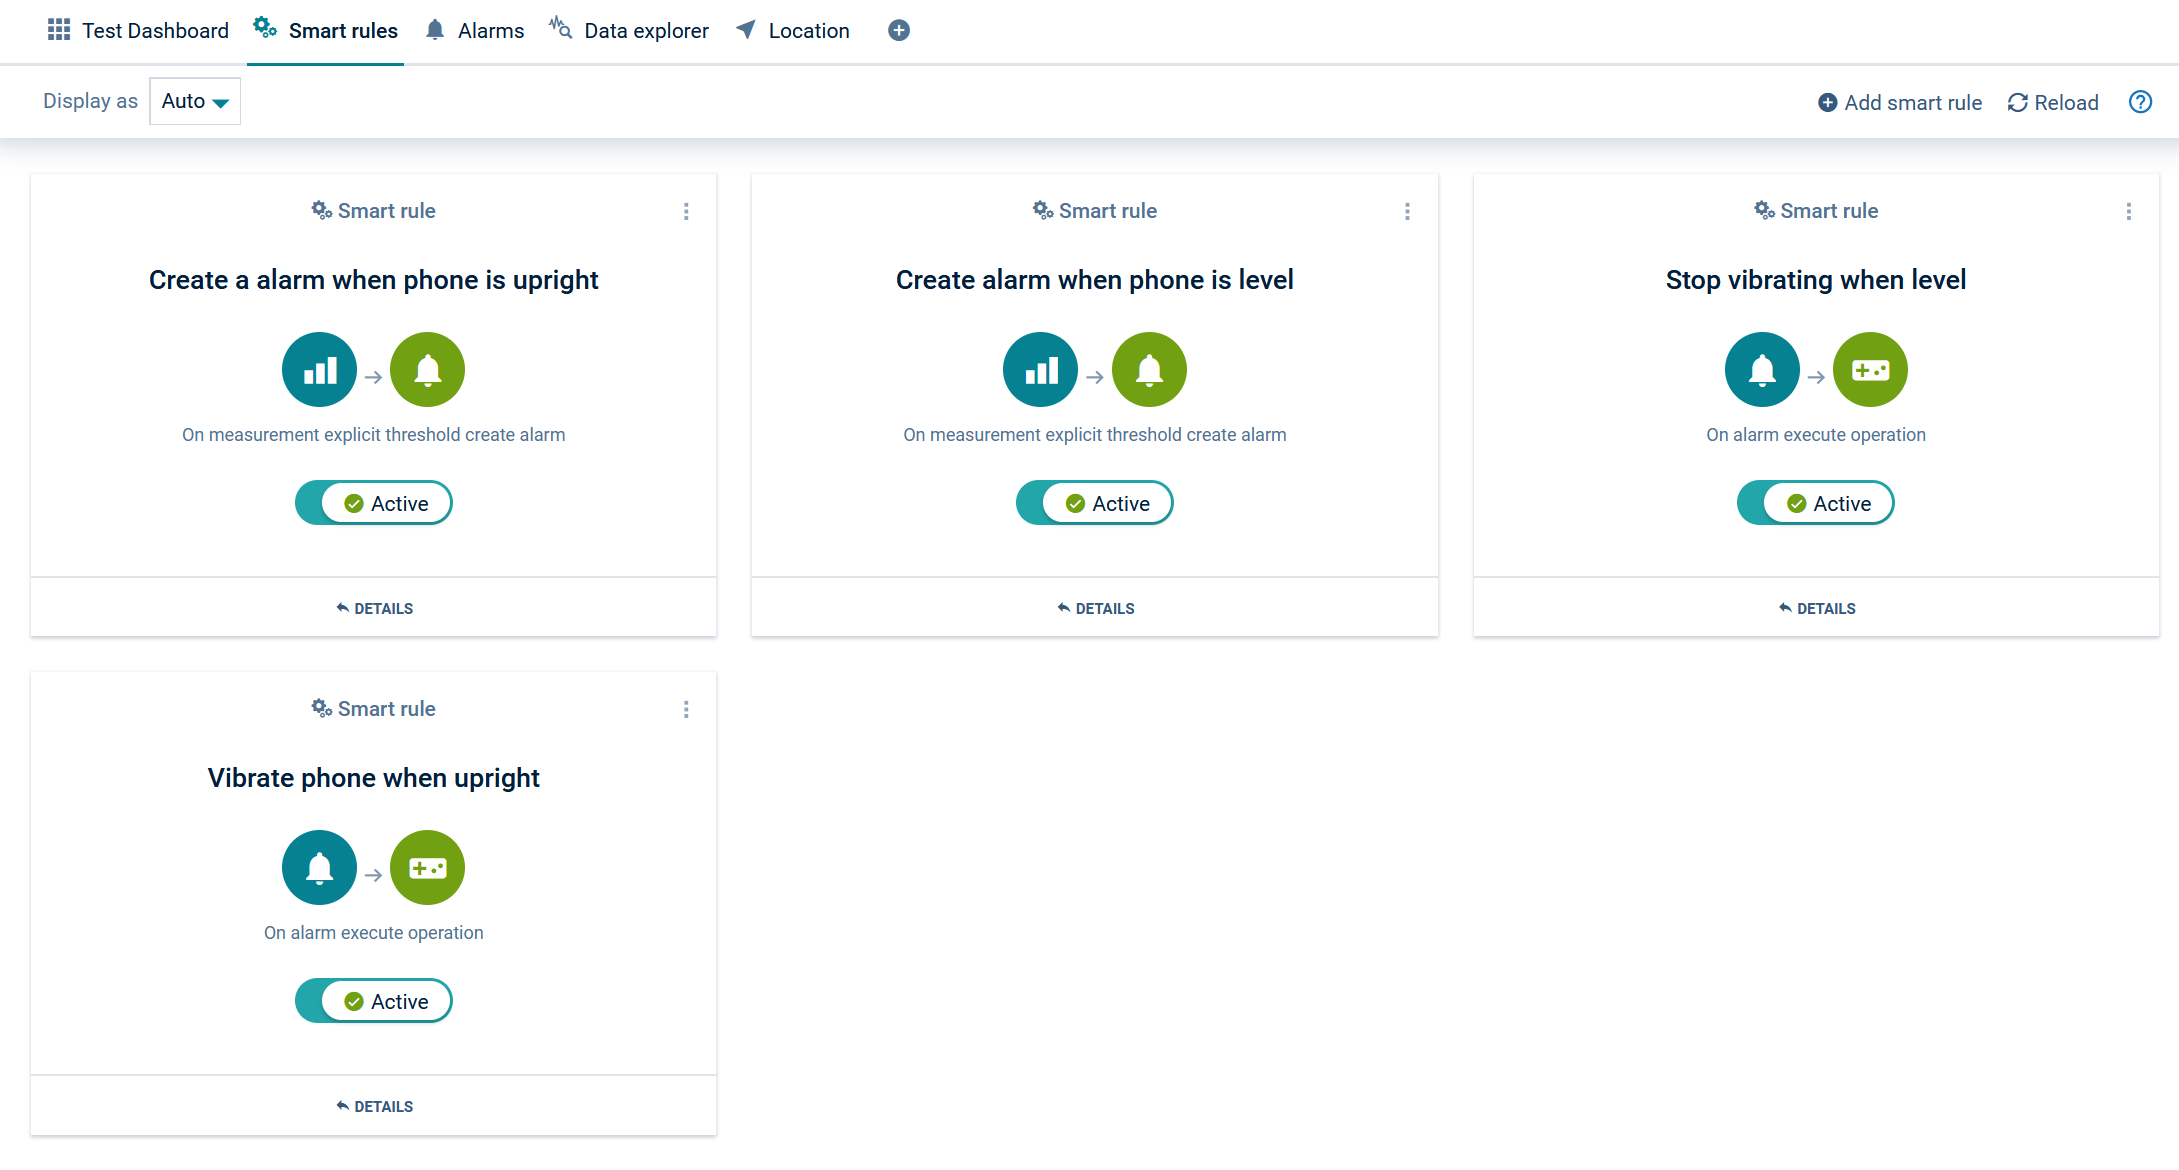
\includegraphics[width=1\textwidth]{exercise_cummolocity/task_2_smart_rules.png}
    \caption{Cumulocity Smart Rule}
    \label{fig:cumulocity_smart_rule}
\end{figure}

\begin{figure}[H]
    \centering
    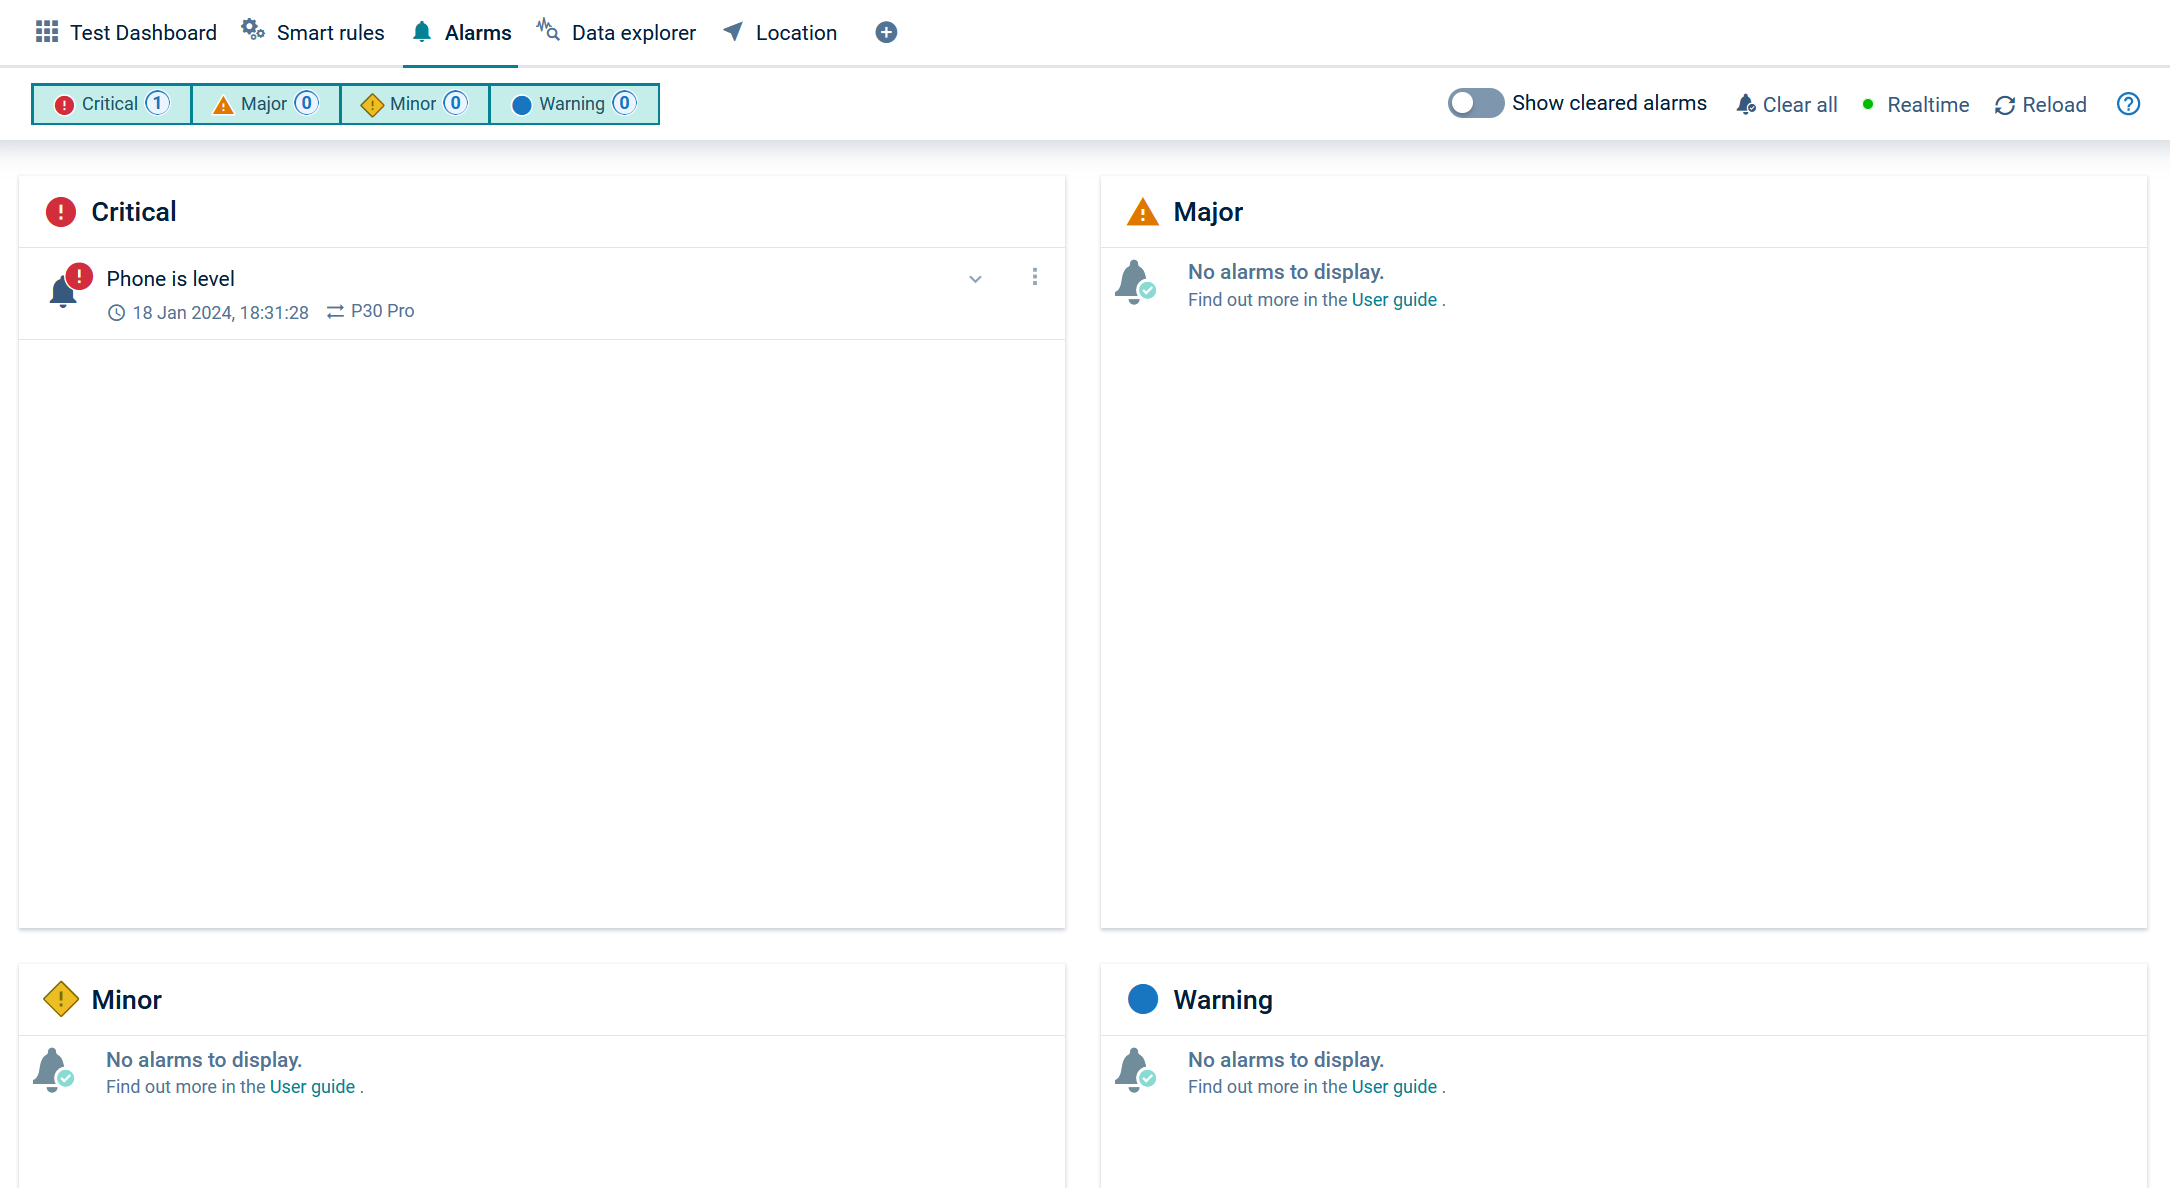
\includegraphics[width=1\textwidth]{exercise_cummolocity/task_2_alarms.png}
    \caption{Cumulocity Alarm}
    \label{fig:cumulocity_alarm}
\end{figure}

\subsection{Task 3: Analytics Builder}

The third task is about creating a analytics builder which could be seen as a more advanced version of the 
smart rules. With the analytics builder you can create more complex rules and also use the data from multiple 
devices and react on this data on a more complex way.
The task was to implement a builder which will detect if the smartphone is shaken and then trigger an alarm.
This was done by using the accelerometer data from the smartphone and a rule which will trigger an alarm if 
the acceleration is above a certain threshold. As before this was straight forward following the instructions 
on the tutorial page.

\begin{figure}[H]
    \centering
    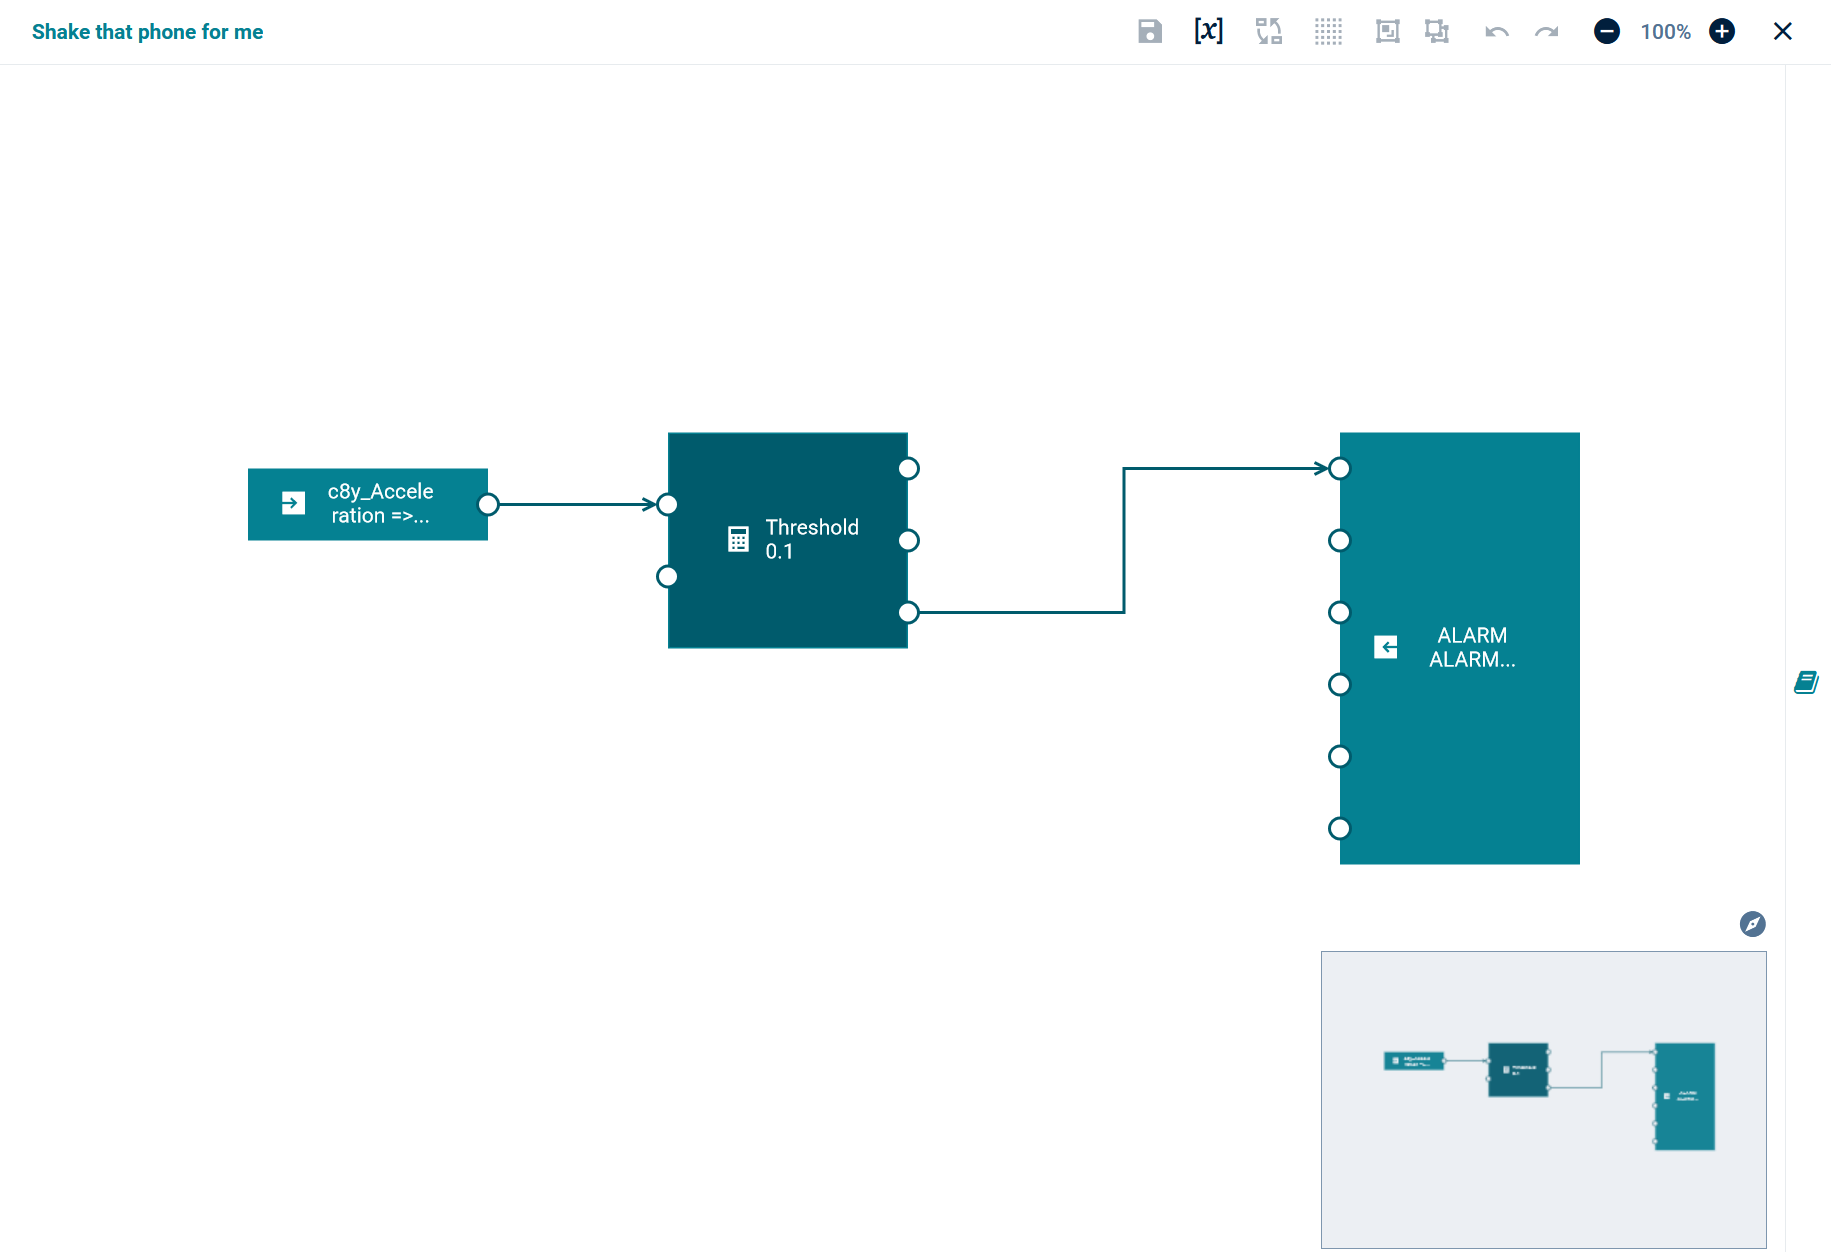
\includegraphics[width=1\textwidth]{exercise_cummolocity/task_3_analytics_builder.png}
    \caption{Cumulocity Analytics Builder}
    \label{fig:cumulocity_analytics_builder}
\end{figure}

\begin{figure}[H]
    \centering
    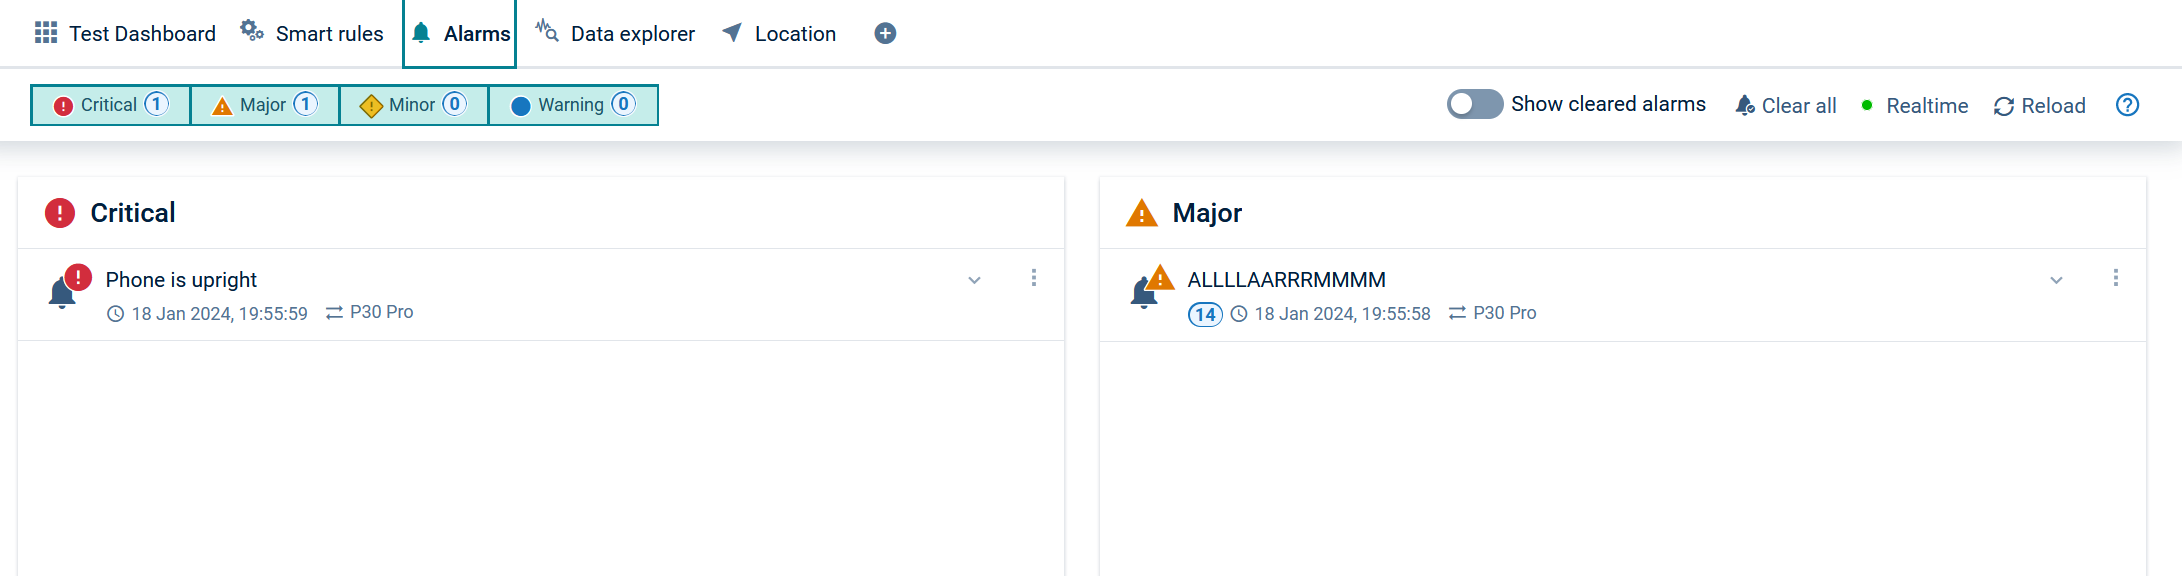
\includegraphics[width=1\textwidth]{exercise_cummolocity/task_3_alarms.png}
    \caption{Cumulocity Alarm}
    \label{fig:cumulocity_alarm}
\end{figure}